\documentclass{article}

\usepackage[%
    left=0.5in,%
    right=0.5in,%
    top=0.5in,%
    bottom=0.5in,%
]{geometry}%
\usepackage{minitoc}
\usepackage{multicol}
\usepackage{graphicx}
\usepackage{fixltx2e}
\usepackage{listings}
\usepackage{color}
\usepackage{hyperref}
    \hypersetup{ colorlinks = true, linkcolor = blue }
\usepackage{blindtext}
\definecolor{lightgray}{gray}{0.9}
\graphicspath{ {./} }

\newcommand{\inlinecode}[2]{\colorbox{lightgray}{\lstinline
[language=#1]$#2$}}
\newcommand{\worddef}[1]{\hyperref[sec:reference]{\textit{#1}}}

\lstset{
  frame=none,
  xleftmargin=2pt,
  stepnumber=1,
  numbers=left,
  numbersep=5pt,
  numberstyle=\ttfamily\tiny\color[gray]{0.3},
  belowcaptionskip=\bigskipamount,
  captionpos=b,
  escapeinside={*'}{'*},
  language=haskell,
  tabsize=2,
  emphstyle={\bf},
  commentstyle=\it,
  stringstyle=\mdseries\rmfamily,
  showspaces=false,
  keywordstyle=\bfseries\rmfamily,
  columns=flexible,
  basicstyle=\small\sffamily,
  showstringspaces=false,
  morecomment=[l]\%,
}
\usepackage{fancyvrb}
\DefineVerbatimEnvironment{code}{Verbatim}{fontsize=\small}

\begin{document}

\tableofcontents

\newpage

\section{Task 1}

\subsection{Repeat until}

\begin{center}
  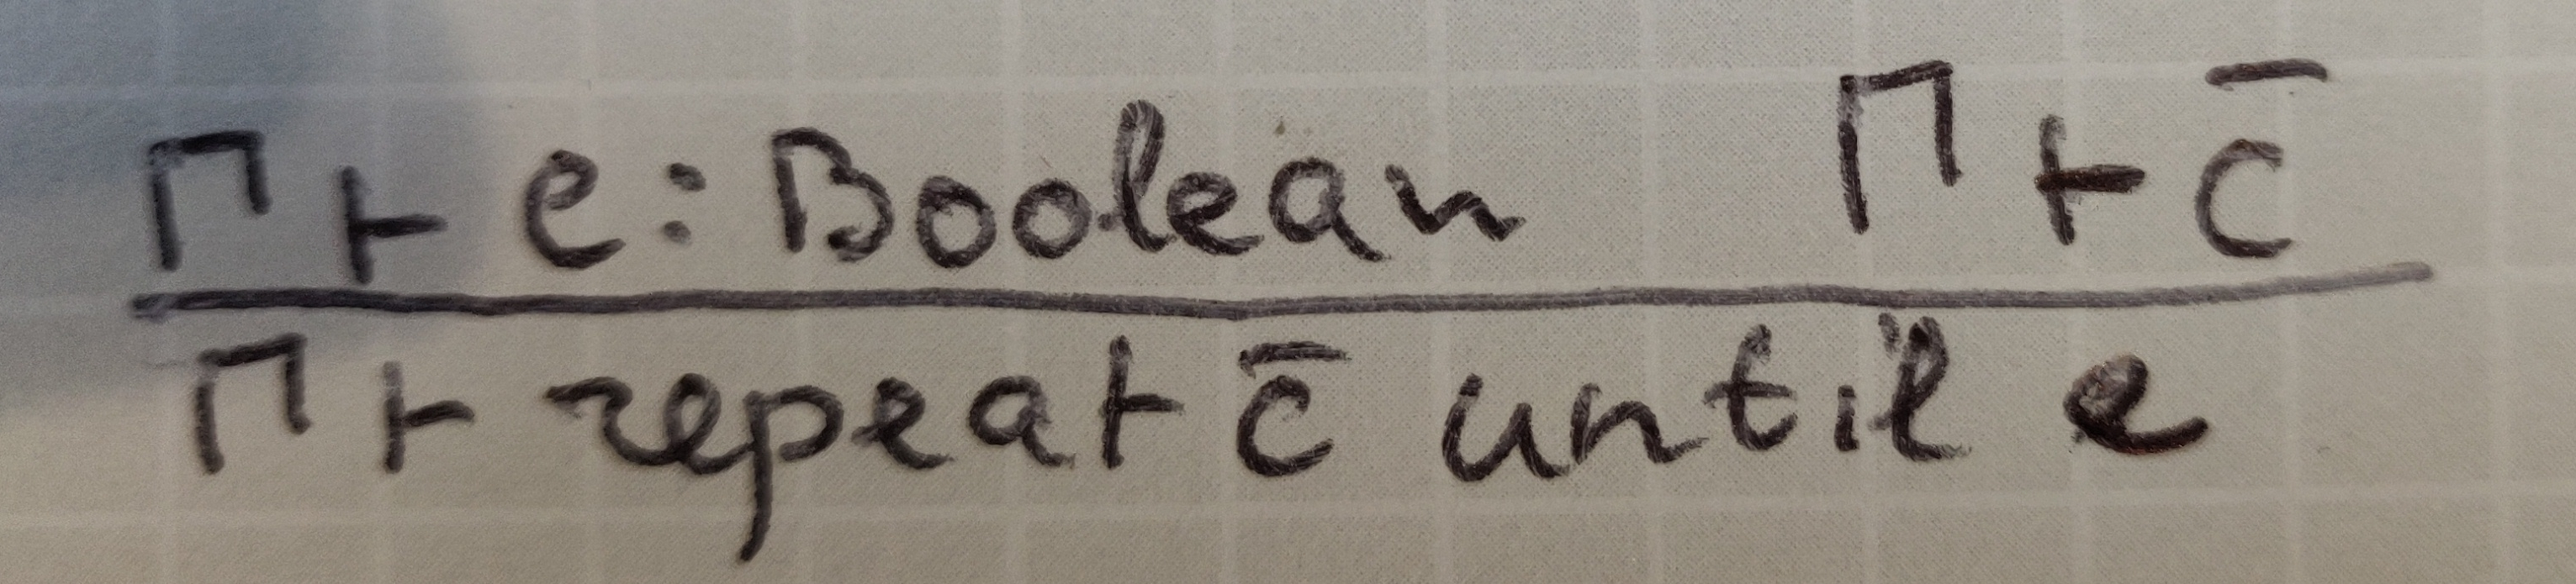
\includegraphics[scale=0.1]{repeat_type.jpg}
\end{center}


\subsection{Character literal}

\begin{center}
  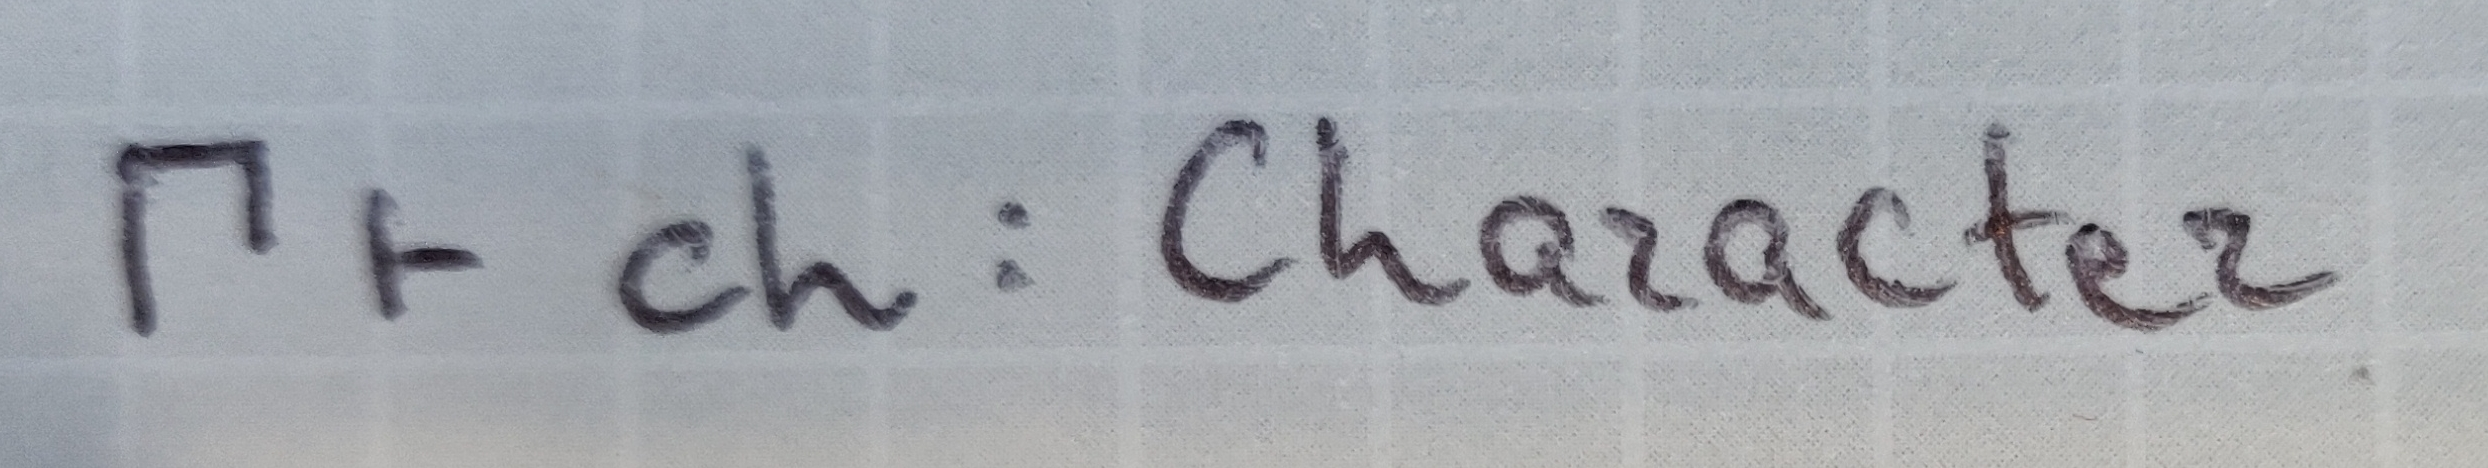
\includegraphics[scale=0.1]{char_type.jpg}
\end{center}


\subsection{If-else extended}

\begin{center}
  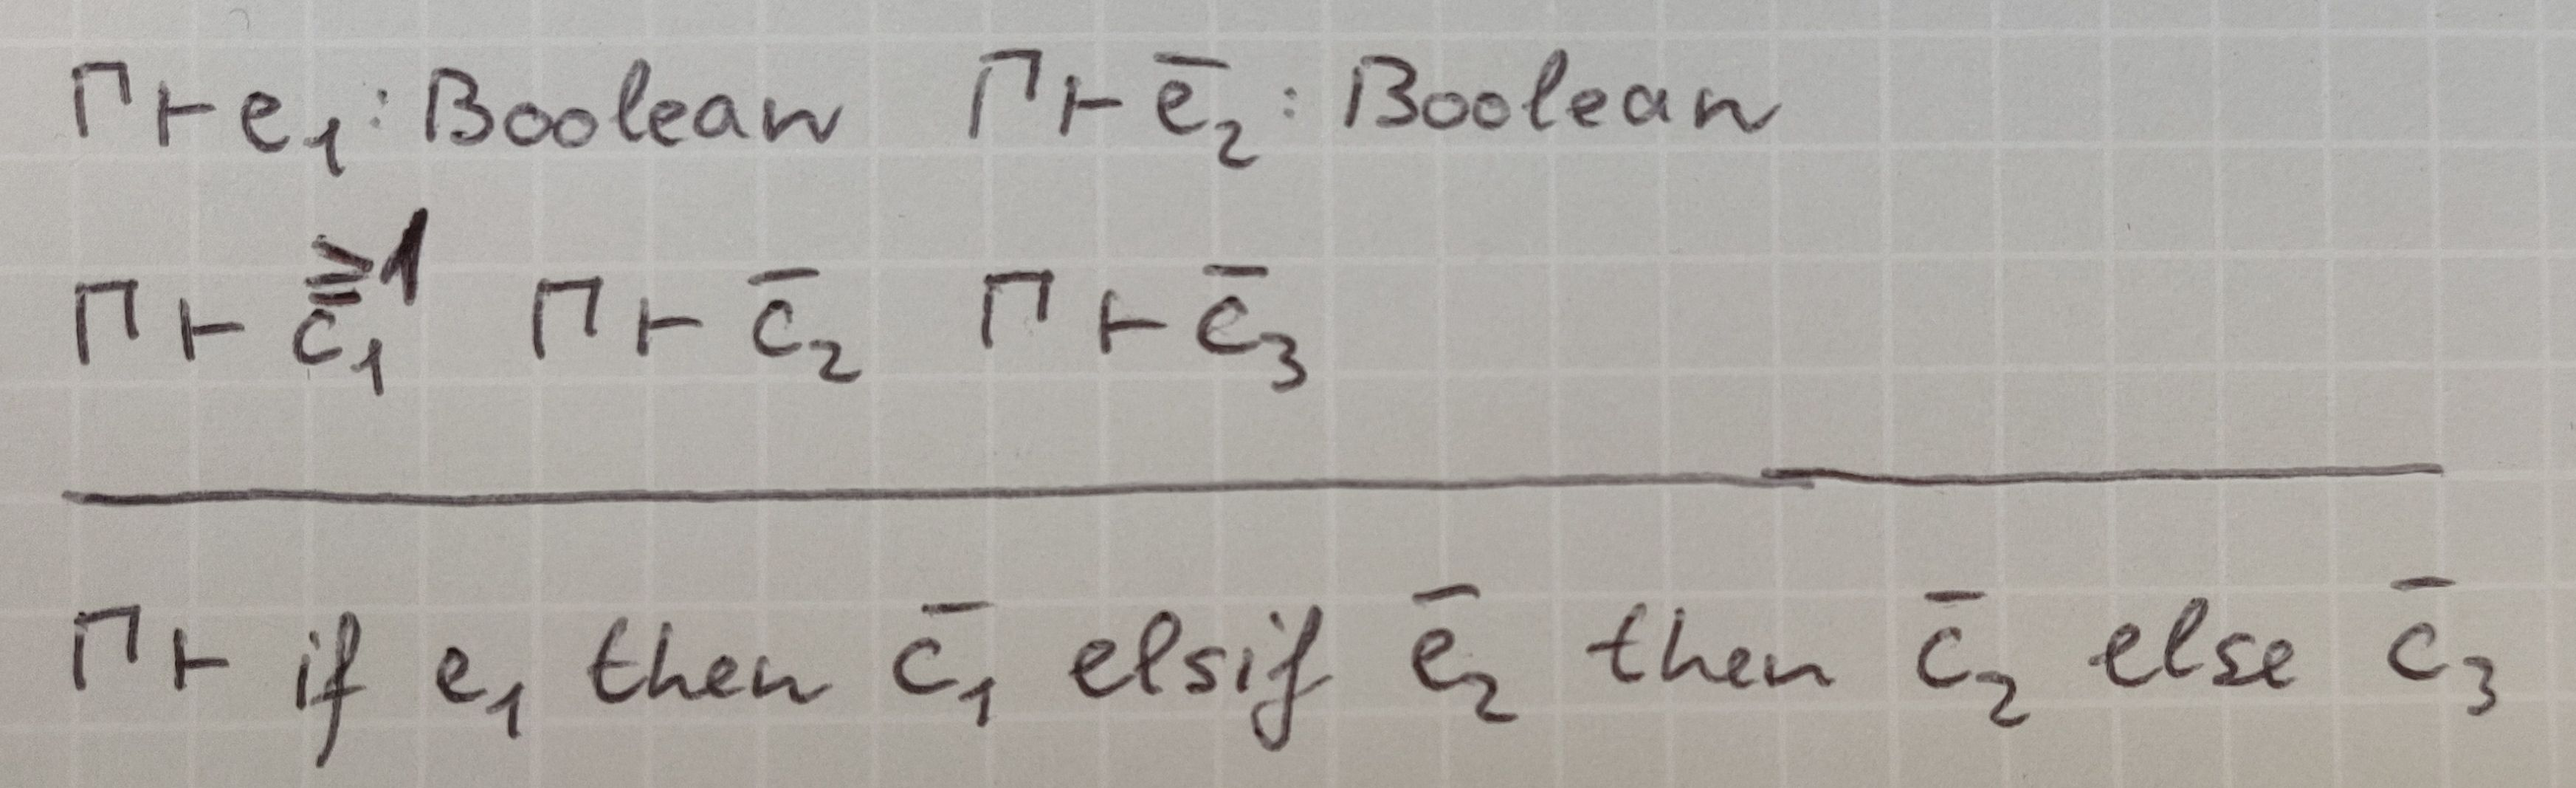
\includegraphics[scale=0.1]{if-else_type.jpg}
\end{center}


\subsection{Conditional expression}

\begin{center}
  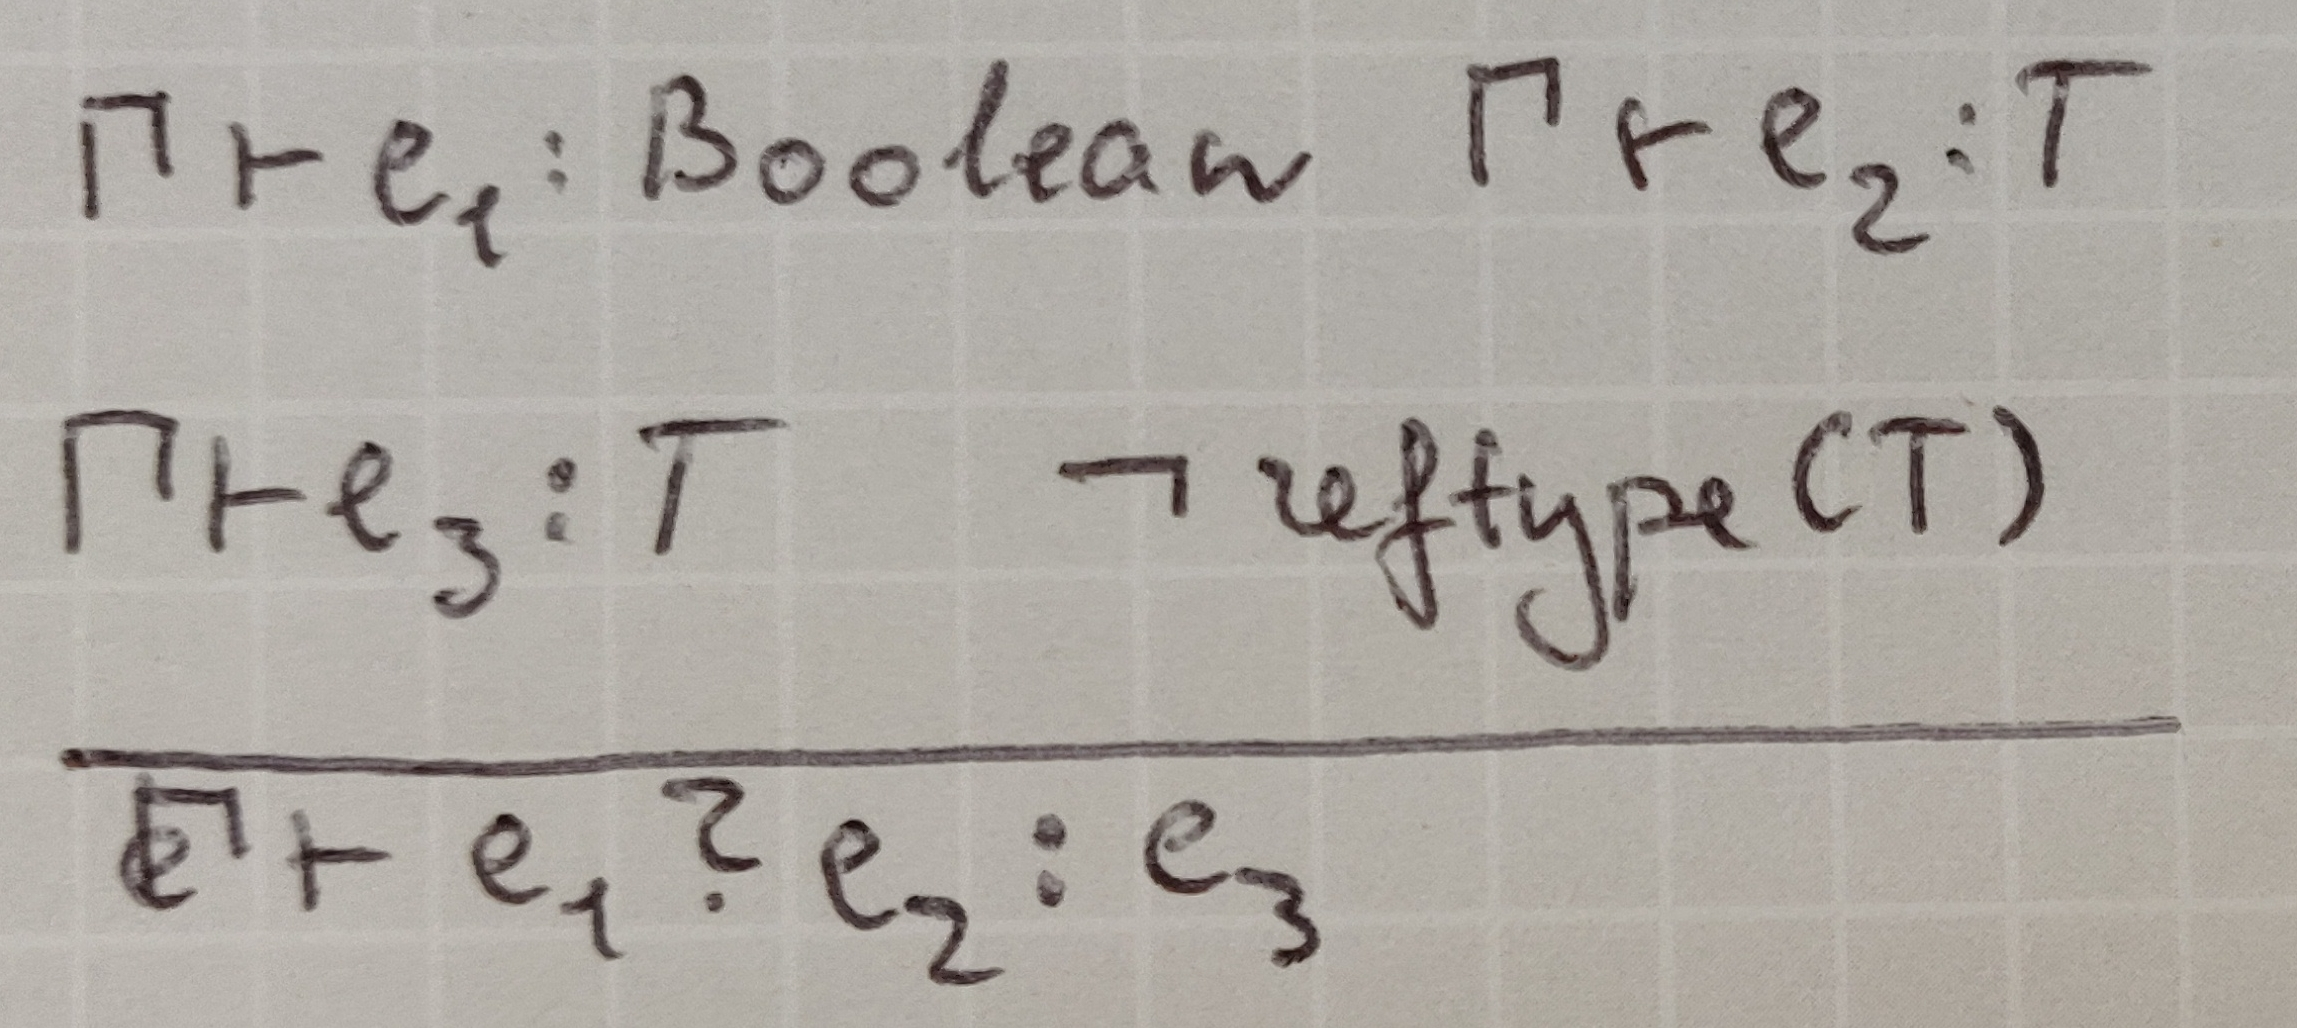
\includegraphics[scale=0.1]{conditional_type.jpg}
\end{center}


\section{Task 2}

\subsection{Repeat until}

\subsubsection{MTIR}

\begin{flushleft}
Update the MiniTriangle Internal Representation inside, so we can stored typed version
\end{flushleft}
\begin{code}
    -- | Repeat until
    | CmdRepeat {
          crCond    :: Expression,      -- ^ Loop-condition
          crBody    :: Command,         -- ^ Loop-body
          cmdSrcPos :: SrcPos
      }
\end{code}

\subsubsection{TypeChecker}
\begin{flushleft}
Add a pattern match for type checking AST \texttt{CmdRepeat} data type
\end{flushleft}
\begin{code}
-- T-REPEAT
chkCmd env (A.CmdRepeat {A.crCond = e, A.crBody = c, A.cmdSrcPos = sp}) = do
    e' <- chkTpExp env e Boolean                        -- env |- e : Boolean
    c' <- chkCmd env c                                  -- env |- c
    return (CmdRepeat {crCond = e', crBody = c', cmdSrcPos = sp})
\end{code}

\subsubsection{PPMTIR}
\begin{flushleft}
Now need a way to print the typed repeat command. We do this by adding a \texttt{CmdRepeat} pattern match to \texttt{ppCommand}
\end{flushleft}
\begin{code}
ppCommand n (CmdRepeat {crCond = e, crBody = c, cmdSrcPos = sp}) =
    indent n . showString "CmdRepeat" . spc . ppSrcPos sp . nl
    . ppCommand (n+1) c
    . ppExpression (n+1) e
\end{code}

\subsection{Character literal}

\subsubsection{Type}

\begin{flushleft}
Firstly we add \texttt{Character} to Type data type
\end{flushleft}
\begin{code}
| Character           -- ^ The Character type
\end{code}
\begin{flushleft}
Next inside \texttt{instance Eq Type where} we add an equality operator pattern for it.
\end{flushleft}
\begin{code}
Character  == Character  = True
\end{code}
\begin{flushleft}
Finally, we add Character pattern match to \texttt{instance Show Type where}
\end{flushleft}
\begin{code}
showsPrec _ Character  = showString "Character"
\end{code}

\subsubsection{TypeChecker}

\begin{flushleft}
We add a \texttt{ExpLitChar} pattern match to \texttt{infTpExp}. The only thing we do here is convert the character value to \texttt{MTChar} and transform $AST \rightarrow MTIR$
\end{flushleft}
\begin{code}
-- T-CHAR
infTpExp env e@(A.ExpLitChr {A.elcVal = c, A.expSrcPos = sp}) = do
    c' <- toMTChr c sp
    return (Character,                          -- env |- n : Character
            ExpLitChr {elcVal = c', expType = Character, expSrcPos = sp})
\end{code}

\subsubsection{MTStdEnv}
\begin{flushleft}
We also need to update our standard environment to contain characters. Do this by updating first list argument in \texttt{mtStdEnv} function
\end{flushleft}
\begin{code}
mtStdEnv :: Env
mtStdEnv =
    mkTopLvlEnv
        [("Boolean",   Boolean),
         ("Integer",   Integer),
         ("Character", Character)]
        [("false",   Boolean, ESVBool False),
         ("true",    Boolean, ESVBool True),
         ("minint",  Integer, ESVInt (minBound :: MTInt)),
         ("maxint",  Integer, ESVInt (maxBound :: MTInt)),
         ("+",       Arr [Integer, Integer] Integer, ESVLbl "add"),
         ("-",       Arr [Integer, Integer] Integer, ESVLbl "sub"),
         ("*",       Arr [Integer, Integer] Integer, ESVLbl "mul"),
         ("/",       Arr [Integer, Integer] Integer, ESVLbl "div"),
         ("^",       Arr [Integer, Integer] Integer, ESVLbl "pow"),
         ("neg",     Arr [Integer] Integer,          ESVLbl "neg"),
         ("<",       Arr [Integer, Integer] Boolean, ESVLbl "lt"),
         ("<=",      Arr [Integer, Integer] Boolean, ESVLbl "le"),
         ("==",      Arr [Integer, Integer] Boolean, ESVLbl "eq"),
         ("!=",      Arr [Integer, Integer] Boolean, ESVLbl "ne"),
         (">=",      Arr [Integer, Integer] Boolean, ESVLbl "ge"),
         (">",       Arr [Integer, Integer] Boolean, ESVLbl "gt"),
         ("&&",      Arr [Boolean, Boolean] Boolean, ESVLbl "and"),
         ("||",      Arr [Boolean, Boolean] Boolean, ESVLbl "or"),
         ("!",       Arr [Boolean] Boolean,          ESVLbl "not"),
         ("getint",  Arr [Snk Integer] Void,         ESVLbl "getint"), 
         ("putint",  Arr [Integer] Void,             ESVLbl "putint"),
         ("skip",    Arr [] Void,                    ESVLbl "skip")]

\end{code}

\subsection{If-else extended}

\subsubsection{MTIR}
\begin{flushleft}
Firstly, we update the internal representation to allow multiple \textit{elsif} and optional \textit{else} branches. Do this by modifying \texttt{CmdIf} inside \texttt{Command} data type.
\end{flushleft}
\begin{code}
-- | Conditional command
| CmdIf {
      ciCondThens :: [(Expression,
                       Command)],   -- ^ Conditional branches
      ciMbElse    :: Maybe Command, -- ^ Optional else-branch
      cmdSrcPos   :: SrcPos
  }
\end{code}

\subsubsection{PPMTIR}
\begin{flushleft}
Now we need to update the pretty print function, so the new syntax can be seen
\end{flushleft}
\begin{code}
ppCommand n (CmdIf {ciCondThens = ecs, ciMbElse = mc, cmdSrcPos = sp}) =
    indent n . showString "CmdIf" . spc . ppSrcPos sp . nl
    . ppSeq (n+1) (\n (e,c) -> ppExpression n e . ppCommand n c) ecs
    . ppOpt (n+1) ppCommand mc
\end{code}

\subsubsection{TypeChecker}
\begin{flushleft}
Next we have to update the command type checking. Do this by updating \texttt{chkCmd} function with:
\end{flushleft}
\begin{code}
-- T-IF
chkCmd env (A.CmdIf {A.ciCondThens = ifs, A.ciMbElse = mbElse,
                     A.cmdSrcPos=sp}) = do
    ifs' <- mapM chkThen ifs
    mbElse' <- case mbElse of
        Nothing -> return Nothing
        Just c -> fmap Just $ chkCmd env c 
    return (CmdIf {ciCondThens = ifs', ciMbElse = mbElse', cmdSrcPos = sp})
    where
        chkThen (e, c) = do
            e' <- chkTpExp env e Boolean
            c' <- chkCmd env c
            return (e', c')
\end{code}
\begin{flushleft}
In the first step we have to go trough the list of our if branches checking each one. We use mapM here in order to make sure list is wrapped in a single monad, rather than having a list of monads. Next we check the optional else branch. To do this properly, we need to make sure that it always returns \texttt{D Maybe} type. If no branch, we just use return function to wrap our Maybe type. If there is a command, we run a check and then map inner contents with a \texttt{Just} type
\end{flushleft}

\subsection{Conditional expression}

\subsubsection{MTIR}
\begin{flushleft}
Firstly add a new data type to Expresion.
\end{flushleft}
\begin{code}
-- | Conditional expression
| ExpCond {
      ecCond    :: Expression,      -- ^ Condition
      ecTrue    :: Expression,      -- ^ Value if condition true
      ecFalse   :: Expression,      -- ^ Value if condition false
      expType    :: Type,           -- ^ Type
      expSrcPos :: SrcPos
  }
\end{code}


\subsubsection{PPMTIR}
\begin{flushleft}
Next we add a way to print the expression to the screen
\end{flushleft}
\begin{code}
ppExpression n (ExpCond {ecCond = c, ecTrue = et, ecFalse = ef, expType = t, expSrcPos = sp})=
    indent n . showString "ExpCond" . spc . ppSrcPos sp . nl
    . ppExpression (n+1) c
    . ppExpression (n+1) et
    . ppExpression (n+1) ef
    . indent n . showString ": " . shows t . nl
\end{code}

\subsubsection{TypeChecker}
\begin{flushleft}
Now we can add a typechecking pattern to \texttt{infTpExp}
\end{flushleft}
\begin{code}
-- T-COND
infTpExp env (A.ExpCond { A.ecCond = c, A.ecTrue = l, A.ecFalse = r, A.expSrcPos = sp }) = do
    c' <- chkTpExp env c Boolean  
    (tl, l') <- infNonRefTpExp env l
    (tr, r') <- infNonRefTpExp env r
    require (tl == tr) sp $ errMsg tl tr
    -- Make sure both types are same and not reference
    return (tl, ExpCond { ecCond = c', ecTrue = l', ecFalse = r', expType = tl, expSrcPos = sp })
    where
        errMsg tl tr = "Expected: " ++ (show tl) ++ " and " ++ (show tr) ++ " types to match"
\end{code}
\begin{flushleft}
We make sure that both types are the same as well as both non-references. Because both are the same we just assign left expression type as the main expression type.
\end{flushleft}

\end{document}
